\documentclass[12pt]{article}%
\usepackage{amsfonts}
\usepackage{fancyhdr}
\usepackage{comment}
\usepackage[a4paper, top=2.5cm, bottom=2.5cm, left=2.2cm, right=2.2cm]%
{geometry}
\usepackage{times}
\usepackage{graphicx}

\usepackage{hyperref}

\usepackage{amssymb}
\usepackage{graphicx}%

\begin{document}

\title{MLT - Assignment 1}
\author{Ayush Sekhari}
\date{\today}
\maketitle

\section{Observations}
\begin{itemize}
\item The data set has missing values
\item Attribute values are numerical - either integers or real numbers
\item Training data is labelled - Supervised Learning 
\item class value 1 is interpreted as "tested positive for diabetes"
\item In my solution, I would be considering Branching factor or Branching Ratio to be 2.
\item The attributes have been renamed as follows : 
\begin{itemize}
\item Number of times pregnant $\rightarrow$ Num\_Preg
\item Plasma glucose concentration a 2 hours in an oral glucose tolerance test $\rightarrow$ PGC
\item Diastolic blood pressure (mm Hg) $\rightarrow$ BP
\item Triceps skin fold thickness (mm) $\rightarrow$ Tricept\_Thickness
\item 2-Hour serum insulin (mu U/ml) $\rightarrow$ Insulin
\item Diabetes pedigree function $\rightarrow$ DPF
\item Age (years) $\rightarrow$ Age
\item Body mass index (weight in kg/(height in m)$^2$) $\rightarrow$ BMI
\item Class variable $\rightarrow$ Label
\end{itemize} 
\item The random seed has been set to 2 for deterministic analysis
\end{itemize}

\section{Libraries Used}
The Programming is done in {\tt R} Programming Language. The following Libraries are used: 
\begin{enumerate}
\item {\tt rpart} : To build, test and plot classification trees
\item {\tt party} : To divide our data-set for 5 fold- cross validation 

\end{enumerate}

\section{Handling Missing Attributes}
The missing data in only in the columns 2-8(Number of times pregnant can be zero).\\
Since the data is numeric, we have to use some substitute for the missing values or handle it in some way(Else, in the case of nominal data, we could have made the missing value as a separate label and classified accordingly). We can handle it in two ways :
\subsection{For Training Data}
parameter : Missing\_Attribute\_Train
\begin{itemize}
\item {\bf Missing\_Attribute\_Train = "UseNA" : } The 0(missing) value is replace by NA in the training data, We do not use this instance while calculating the impurity with respect to this attribute for finding the splitting criteria. 
\item {\bf Missing\_Attribute\_Train = "UseMean" : } The 0(missing) value is replaced by the class average for that corresponding attribute in the training data. Class average seems to be a better substitute as compared to total average. We can replace by other metrics as well like median or mode but I would be using mean. 
\end{itemize}

\subsection{For Test Data}
parameter : Missing\_Attribute\_Test
\begin{itemize}
\item {\bf Missing\_Attribute\_Test = "UseNA" : } The 0(missing) value is replace by NA in the training data, We use surrogate splits to estimate in the cases where the missing attribute is required for splitting. These surrogate splits were calculated while training. 

\item {\bf Missing\_Attribute\_Test = "UseMean" : } The 0(missing) value is replaced by the class average for that corresponding attribute in the training data. Training data is used instead of test data because we don't know much about the test data, test data in real life is very small and given tuple wise. Class average seems to be a better substitute as compared to total average. We can replace by other metrics as well like median or mode but I would be using mean. 
\end{itemize}
\section{5 Fold Cross-Validation}
We have randomly divided our data set into 5 disjoint (approximately same size) data sets. 
One part is used as the test set and other is used as the training set. 

\section{Paramters Used}
The following Parameters signify the conditions in which the classification tree was constructed on training data and performance was measured on test data.
\begin{itemize}
\item {\bf Impurity\_Function (I) } : may be "gini" for gini index or "information" for entropy as the impurity function
\item {\bf Missing\_Attributes\_Train (MATr)} : may be "useNA" or "useMean"
\item {\bf Missing\_Attributes\_Test(MATe)} : may be "useNA" or "useMean"
\end{itemize}


\section{Grow the tree as much as possible and then Prune}
Script Used : {\tt Pruning.R} \\

Here for each cross validation set iteration, we first build a completely overfitting tree for the training data by setting the parameters cp = 0 and minsplit = 1 .\\
The we pruned the tree using the value of cp for which {\tt X-Val Relative} error is the minimum. This is done using the cptable data of the decision tree. Help was taken from the online source \url{http://www.statmethods.net/advstats/cart.html} \\
The Plot of X-val relative vs CP for the training set 5 is as shown in figure \ref{fig:xvalvscp}. The minima in this graph is used for the value of cp at which pruning is done. \\
\begin{figure}[h!]

  \caption{X-val Relative Error vs CP for training set 5}
  \centering
    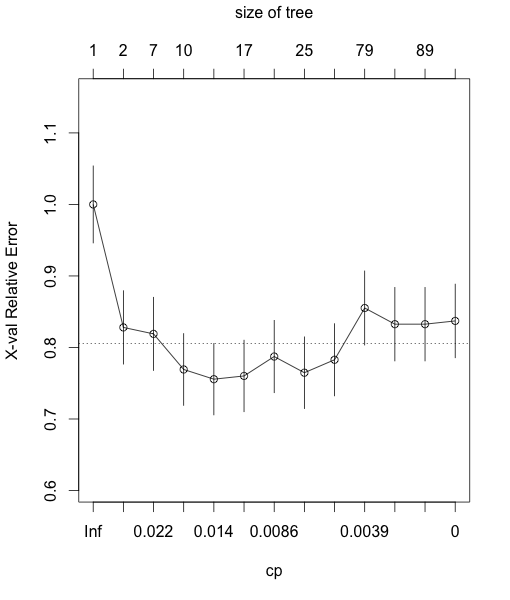
\includegraphics[width=0.7\textwidth]{xval_vs_cp_5}
    \label{fig:xvalvscp}
\end{figure}
 
Various Performance metrics under different cases are as shown in Tables below.
 
\begin{center}
\begin{table}
\centering
\label{table:prune}
\caption{Various Performance metrics under different parameters while pruning}
\begin{tabular}{|p{2in}|c|c|c|c|c|c|}
 \hline
 {\bf Parameters } & {\bf accuracy } & {\bf precision } & {\bf recall } & {\bf TP Rate } & {\bf FP Rate } & {\bf F1 Score } \\ \hline
 {\bf I = gini MATr = UseNA MATe = UseNA } & {\bf 0.753 } & {\bf 0.686 } & {\bf 0.562 } & {\bf 0.562 } & {\bf 0.14 } & {\bf 0.61 } \\ \hline
  {\bf I = information MATr = UseNA MATe = UseNA } & {\bf 0.741 } & {\bf 0.658 } & {\bf 0.577 } & {\bf 0.577 } & {\bf 0.169 } & {\bf 0.606 } \\ \hline
  {\bf I = gini MATr = UseMean MATE = UseNA}& {\bf 0.725 } & {\bf 0.623 } & {\bf 0.548 } & {\bf 0.548 } & {\bf 0.179 } & {\bf 0.581 } \\ \hline
  {\bf I = information MATr = UseMean MATE = UseNA} & {\bf 0.732 } & {\bf 0.628 } & {\bf 0.557 } & {\bf 0.557 } & {\bf 0.175 } & {\bf 0.589 } \\ \hline
{\bf I = gini , MATr = UseNA , MATe = UseMean  } & {\bf 0.74 } & {\bf 0.677 } & {\bf 0.512 } & {\bf 0.512 } & {\bf 0.134 } & {\bf 0.575 } \\ \hline
{\bf I = information , MATr = UseNA , MATe = UseMean  } & {\bf 0.737 } & {\bf 0.655 } & {\bf 0.56 } & {\bf 0.56 } & {\bf 0.167 } & {\bf 0.596 } \\ \hline
{\bf I = gini , MATr = UseMean , MATe = UseMean  } & {\bf 0.697 } & {\bf 0.672 } & {\bf 0.26 } & {\bf 0.26 } & {\bf 0.07 } & {\bf 0.374 } \\ \hline
{\bf I = information , MATr = UseMean , MATe = UseMean  } & {\bf 0.704 } & {\bf 0.644 } & {\bf 0.33 } & {\bf 0.33 } & {\bf 0.096 } & {\bf 0.426 } \\ \hline

\end{tabular}
\end{table}
\end{center}

\section{Threshold on the number of data vectors at a node while splitting}
Script Used : {\tt MinSplit.R} \\ 
We alter the {\tt minsplit} parameter in {\tt rpart.control} to set the minimum number of observations that must exist in a node in order for a split to be attempted while building the classification tree.
Here, we divide the data into 4:1 parts, training is done on the larger part and we chose the value of the parameter for which accuracy on the test data is the best. We have used the average obtained in this way. (It was seen after dividing the data into three parts i.e. CV +  Test +  Train, that our model performs good). The parameter {\tt cp} is set to be 0 for independent effects of minsplit.  Final accuracies are though reported using 5 Fold Cross-Validation. Various performance metrics under different parameter settings can be seen in the tables below.

\begin{center}
\begin{table}
\centering
\label{table:prune}
\caption{Various Performance metrics under different parameters while using threshold on the number of data vectors at a node while splitting}
\begin{tabular}{|p{2in}|c|c|c|c|c|c|}
 \hline
 {\bf Parameters } & {\bf accuracy } & {\bf precision } & {\bf recall } & {\bf TP Rate } & {\bf FP Rate } & {\bf F1 Score } \\ \hline
 {\bf I = gini , MATr = UseNA , MATe = UseNA  } & {\bf 0.78 } & {\bf 0.705 } & {\bf 0.628 } & {\bf 0.628 } & {\bf 0.14 } & {\bf 0.661 } \\ \hline
 {\bf I = information , MATr = UseNA , MATe = UseNA  } & {\bf 0.783 } & {\bf 0.69 } & {\bf 0.687 } & {\bf 0.687 } & {\bf 0.167 } & {\bf 0.688 } \\ \hline
 {\bf I = gini , MATr = UseMean , MATe = UseNA  } & {\bf 0.736 } & {\bf 0.64 } & {\bf 0.606 } & {\bf 0.606 } & {\bf 0.192 } & {\bf 0.613 } \\ \hline
 {\bf I = information , MATr = UseMean , MATe = UseNA  } & {\bf 0.738 } & {\bf 0.641 } & {\bf 0.598 } & {\bf 0.598 } & {\bf 0.185 } & {\bf 0.612 } \\ \hline
{\bf I = gini , MATr = UseNA , MATe = UseMean  } & {\bf 0.773 } & {\bf 0.705 } & {\bf 0.601 } & {\bf 0.601 } & {\bf 0.136 } & {\bf 0.644 } \\ \hline
{\bf I = information , MATr = UseNA , MATe = UseMean  } & {\bf 0.78 } & {\bf 0.689 } & {\bf 0.679 } & {\bf 0.679 } & {\bf 0.167 } & {\bf 0.684 } \\ \hline
{\bf I = gini , MATr = UseMean , MATe = UseMean  } & {\bf 0.715 } & {\bf 0.685 } & {\bf 0.364 } & {\bf 0.364 } & {\bf 0.102 } & {\bf 0.464 } \\ \hline
{\bf I = information , MATr = UseMean , MATe = UseMean  } & {\bf 0.713 } & {\bf 0.678 } & {\bf 0.355 } & {\bf 0.355 } & {\bf 0.094 } & {\bf 0.453 } \\ \hline

\end{tabular}
\end{table}
\end{center}

\section{Threshold on the decrease in impurity while splitting}
Script Used : {\tt Decrease.R} \\ 
We alter the {\tt cp} parameter in {\tt rpart.control}. Any split that does not decrease the overall lack of fit by a factor of {\tt cp} is not attempted. 
Here, we divide the data into 4:1 parts, training is done on the larger part and we chose the value of the parameter for which accuracy on the test data is the best. We have used the average obtained in this way. (It was seen after dividing the data into three parts i.e. CV +  Test +  Train, that our model performs good). The parameter {\tt minsplit} is set to be 1 for independent effects of cp. Final accuracies are though reported using 5 Fold Cross-Validation. Various performance metrics under different parameter settings can be seen in the tables below. 
\begin{center}
\begin{table}
\centering
\label{table:prune}
\caption{Various Performance metrics under different parameters while using threshold on the decrease in impurity while splitting}
\begin{tabular}{|p{2in}|c|c|c|c|c|c|}
 \hline
 {\bf Parameters } & {\bf accuracy } & {\bf precision } & {\bf recall } & {\bf TP Rate } & {\bf FP Rate } & {\bf F1 Score } \\ \hline
 {\bf I = gini , MATr = UseNA , MATe = UseNA  } & {\bf 0.771 } & {\bf 0.689 } & {\bf 0.628 } & {\bf 0.628 } & {\bf 0.152 } & {\bf 0.655 } \\ \hline
 {\bf I = information , MATr = UseNA , MATe = UseNA  } & {\bf 0.767 } & {\bf 0.72 } & {\bf 0.569 } & {\bf 0.569 } & {\bf 0.124 } & {\bf 0.62 } \\ \hline
 {\bf I = gini , MATr = UseMean , MATe = UseNA  } & {\bf 0.742 } & {\bf 0.634 } & {\bf 0.647 } & {\bf 0.647 } & {\bf 0.205 } & {\bf 0.635 } \\ \hline
 {\bf I = information , MATr = UseMean , MATe = UseNA  } & {\bf 0.743 } & {\bf 0.644 } & {\bf 0.595 } & {\bf 0.595 } & {\bf 0.177 } & {\bf 0.616 } \\ \hline
{\bf I = gini , MATr = UseNA , MATe = UseMean  } & {\bf 0.758 } & {\bf 0.682 } & {\bf 0.576 } & {\bf 0.576 } & {\bf 0.146 } & {\bf 0.619 } \\ \hline
{\bf I = information , MATr = UseNA , MATe = UseMean  } & {\bf 0.766 } & {\bf 0.732 } & {\bf 0.531 } & {\bf 0.531 } & {\bf 0.106 } & {\bf 0.604 } \\ \hline
{\bf I = gini , MATr = UseMean , MATe = UseMean  } & {\bf 0.714 } & {\bf 0.679 } & {\bf 0.363 } & {\bf 0.363 } & {\bf 0.104 } & {\bf 0.463 } \\ \hline
{\bf I = information , MATr = UseMean , MATe = UseMean  } & {\bf 0.711 } & {\bf 0.651 } & {\bf 0.377 } & {\bf 0.377 } & {\bf 0.109 } & {\bf 0.468 } \\ \hline
\end{tabular}
\end{table}
\end{center}

\section{Conclusions}
In General the average accuracy observed is between 72-77\%. This is quite good with such simple models.
\end{document}
